\documentclass[12pt,aspectratio=169]{beamer}

\mode<presentation>
{
  \usetheme{Singapore}
 %\setbeamersize{text margin left=.6cm,text margin right=.6cm}
%  \setbeamertemplate{navigation symbols}{} % suppress nav bar
%  \setbeamercovered{transparent}
}
\usefonttheme{professionalfonts}
\usepackage{graphicx}
\usepackage{tikz}
\usepackage{amsmath}
\usepackage{mathpazo}
\usepackage[scaled]{helvet}
\usepackage{xcolor,colortbl}
\usepackage{siunitx}
\usepackage[siunitx]{circuitikz} % to draw circuits!

\sisetup{
  number-math-rm=\mathnormal,
  per-mode=symbol
}

\title{Classes 14: Magnetism, Part 2}
\subtitle{AP Physics}
\author[TML]{Dr.\ Timothy Leung}
\institute{Olympiads School}
\date{February 2018}

\newcommand{\pic}[2]{\includegraphics[width=#1\textwidth]{#2}}
\newcommand{\mb}[1]{\mathbf{#1}}
\newcommand{\eq}[2]{\vspace{#1}{\Large\begin{displaymath}#2\end{displaymath}}}
\newcommand{\protip}[1]{
  \begin{center}
    \fbox{
      \begin{minipage}{.95\textwidth}
        {\footnotesize
          \textbf{Protip: }#1
        }
      \end{minipage}
    }
  \end{center}
}

\begin{document}

\begin{frame}
  \maketitle
\end{frame}


%\section[Intro]{Introduction}

\begin{frame}
  \frametitle{Files for You to Download}
  Download from the school website:
  \begin{enumerate}
  \item\texttt{14-Magnetism2.pdf}---The ``print version'' of this
    presentation. If you want to print the slides on paper, I recommend
    printing 4 slides per page.
%  \item\texttt{14-Homework.pdf}---Homework assignment for Class 14.
%    Please note the new formatting style
  \end{enumerate}

  \vspace{.2in}Please download/print the PDF file before each class. When you
  are taking notes, pay particular attention to things I say that aren't
  necessarily on the slides.
\end{frame}

\section{Amp\`{e}re's Law}

\begin{frame}
  \frametitle{Amp\`{e}re's Law}
  \begin{columns}
    \column{.25\textwidth}
    \pic{1}{amlaw.png}
    
    \column{.75\textwidth}
    Like Gauss's law to calculate electric fields for symmetric configurations,
    \textbf{Amp\`{e}re's law} can be used to calculate the magnetic field for
    symmetric configurations:

    \eq{-.1in}{\boxed{\oint_C \mb{B}\cdot d\boldsymbol{\ell}=\mu_o I_C}}
    where
    \begin{itemize}
    \item $C$ is a closed curve around a current (``Amperian lop'')
    \item $d\boldsymbol{\ell}$ is an infinitesimal length along the closed curve
    \item $I_c$ is the net current that penetrates the area bounded by $C$
    \end{itemize}
  \end{columns}
\end{frame}

\begin{frame}
  \frametitle{Application of Amp\`{e}re's Law: Infinitely Long Wire}
  \begin{columns}
    \column{.3\textwidth}
    \pic{1}{4iM3O.jpg}

    \column{.7\textwidth}
    An \emph{infinitely} long wire must generate a magnetic field that only
    depend on radial distance. We place our loop as a circle of radius $r$
    around the wire. Amp\`{e}re's law reduces to:

    \eq{-.3in}{
      \oint_C \mb{B}\cdot d\boldsymbol{\ell}=\mu_o I_C
      \;\rightarrow\;
      B(2\pi r)=\mu_o I
    }
      
    From this, we get our expression of the magnetic field from an infinitely
    long wire:
      
    \eq{-.25in}{
      B=\frac{\mu_o I}{2\pi r}
    }
  \end{columns}
\end{frame}


\begin{frame}
  \frametitle{Toroid}
  \begin{columns}
    \column{.3\textwidth}
    \pic{1.15}{toroid.png}

    {\scriptsize A toroid consists of a current-\\
      carrying wire wound around a donut-shaped core \par}
    
    \column{.7\textwidth}
    Another application of Amp\`{e}re's Law is the \textbf{toroid}. This time,
    we put our loop at $a<r<b$ inside the toroid. Once again, because of
    symmetry, Amp\`{e}re's law reduces to:

    \vspace{-.35in}{\Large
      \begin{align*}
        \oint_C \mb{B}\cdot d\boldsymbol{\ell}&=\mu_o I_C\\
        B(2\pi r)&=\mu_o NI\\
        B&=\frac{\mu_o NI}{2\pi r}
      \end{align*}
    }

    \vspace{-.15in}where $N$ is the number of times the wire is wound around
    the core
    
  \end{columns}
\end{frame}


\begin{frame}
  \frametitle{Toroid}
  \begin{columns}
    \column{.3\textwidth}
    \pic{1.15}{toroid.png}

    \column{.7\textwidth}
    More interestingly, when the loop is placed at $r<a$:

    \eq{-.3in}{B=0\quad\text{for}\quad r<a}

    \vspace{-.2in}When the loop is placed at $r>b$, the amount of current
    penetrating the loop is the same in both direction, i.e.\ $I_c=0$, and

    \eq{-.4in}{B=0\quad\text{for}\quad r>b}
    
    \vspace{-.2in}In fact, the \emph{only} place that a magnetic field exists
    is inside the core, between $a$ and $b$, where 
    
    \eq{-.2in}{
      B=\frac{\mu_o NI}{2\pi r}\quad\text{for}\quad a\leq r\leq b
    }
  \end{columns}
\end{frame}


%\begin{frame}
%  \frametitle{Upcoming homework}
%
%  Your upcoming homework will have a couple of questions for applying
%  Amp\`{e}re's law for common configurations.
%\end{frame}

\section{Faraday's Law}

\begin{frame}
  \frametitle{Magnetic Flux}

  \textbf{Question:} If a current-carrying wire can generate a magnetic field,
  can a magnetic field affect the current in a wire?

  \vspace{.3in}\textbf{Answer:} Yes, sort of\ldots

  \vspace{.3in}To understand how to \emph{induce} a current by a magnetic field,
  we need to look at fluxes again.
\end{frame}

\begin{frame}
  \frametitle{Magnetic Flux}
  \begin{columns}
    \column{.4\textwidth}
    \pic{1.1}{flux2.png}
  
    \column{.6\textwidth}
    Magnetic flux is defined as:
    
    \eq{-.15in}{
      \boxed{\Phi_\mathrm{magnetic}=\int\mb{B}\cdot d\mb{A}}
    }
    
    \vspace{-.1in}where $\mb{B}$ is the magnetic field, and $d\mb{A}$ is the
    infinitesimal area pointing \textbf{outwards}. If you are uncomfortable
    with using vector surfaces, note that magnetic flux can also be expressed
    as:

    \eq{-.15in}{
      \boxed{\Phi_\mathrm{magnetic}=\int\mb{B}\cdot\hat{\mb{n}}dA}
    }

    \vspace{-.1in}where $\hat{\mb{n}}$ is the outward normal direction
  \end{columns}
\end{frame}


\begin{frame}
  \frametitle{Magnetic Flux Over a Closed Surface}

  The unit for magnetic flux is a ``weber'' (\si{\weber}), in honor of
  German physicist Wilhelm Weber, who invented the electromagnetic
  telegraph with Carl Gauss. The unit is defined as:

  \eq{-.3in}{\SI{1}{\weber}=\SI{1}{\tesla.\metre^2}}
  
  \vspace{-.2in}The magnetic flux over a closed surface is always zero:

  \eq{-.2in}{
    \boxed{\oint\mb{B}\cdot d\mb{A}=0}
  }

  \vspace{-.1in}Since magnetic field lines only exist as a loop, that means
  there should be equal amount of ``flux'' flowing out of a closed surface as
  entering the surface.
\end{frame}

\begin{frame}
  \frametitle{When Magnetic Flux is Changing}

  \begin{itemize}
  \item When the magnetic flux $\Phi_{\textrm{magnetic}}$ is changing, an
    electromotive force (\emph{emf}, $\mathcal{E}$) is created in the wire.
  \item Unlike in a circuit, where the \emph{emf} is concentrated at the
    terminals of the battery, the induced \emph{emf} is spread across the
    entire wire.
  \end{itemize}
  \begin{columns}
    \column{.3\textwidth}
    \begin{center}
      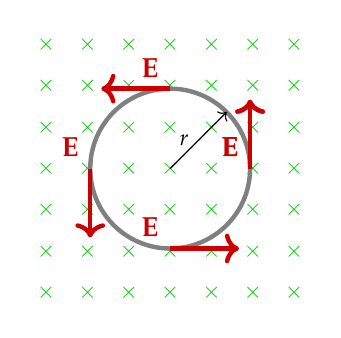
\begin{tikzpicture}[scale=.35]
        \foreach \xx in {-4.5,-3,...,4.5}{
          \foreach \yy in {-4.5,-3,...,4.5}{
            \node at (\xx,\yy) {\footnotesize\textcolor{green!80!black}{$\times$}};
          }
        }
        \draw[gray,ultra thick](0,0) circle(2.9);
        \draw[->,rotate=45](0,0)--(2.9,0) node[midway,left]{\footnotesize $r$};
        \foreach \x in {0,90,...,360} {
          \begin{scope}[rotate=\x]
            \draw[ultra thick,red!80!black,->](2.9,0)--(2.9,2.5)
            node[pos=0,above left]{$\mb{E}$};
          \end{scope}
        }
      \end{tikzpicture}
    \end{center}
    
    \column{.7\textwidth}
    \begin{itemize}
    \item Since \emph{emf} is work per unit charge, that means that there is an
      electric field inside the wire to move the charges.
    \item In this example:
      \begin{itemize}
      \item Magnetic field $\mb{B}$ into the page
      \item The direction of the electric field $\mb{E}$ corresponds to an
        \emph{increase} in magnetic flux
      \end{itemize}
    \end{itemize}
  \end{columns}
\end{frame}


\begin{frame}
  \frametitle{Faraday's Law}
  Faraday's law states that the rate of change of magnetic flux produces an
  electromotive force:

  \eq{-.3in}{
    \boxed{
      \mathcal{E}=\oint\mb{E}\cdot d\mb{l}={\color{red}{-}}\frac{d\Phi}{dt}
    }
  }
  
  The negative sign {\textcolor{red}{highlighted in red}} is the result of
  Lenz's law, which is related to the conservation energy
\end{frame}


%\begin{frame}
%  \frametitle{Example Problem}
%  \textbf{Example:} A magnetic field $\mb{B}$ is perpendicular to the plane of
%  the page, and uniform in a circular region of radius $R$ as shown. Outside of
%  the circular region, $\mb{B}=\mb{0}$. The rate of change of the magnitude of
%  $\mb{B}$ is $dB/dt$. What is the magnitude of the induced electric field in 
%  the plane of the page at a distance $r$ from the center of the circular
%  region?
%\end{frame}


\begin{frame}
  \frametitle{How Can Magnetic Flux Change}
  Magnetic flux can change due to a number of reasons:
  \begin{enumerate}
  \item\textbf{Changing magnetic field strength} e.g.\  if $\mb{B}$ is created
    by a time dependent current source like an alternating current
  \item\textbf{Changing orientation of magnetic field} because the
    surface area is moving (translation and/or rotation) relative to $\mb{B}$
  \item\textbf{Changing area} the surface area from which the flux is
    calculated is changing
  \end{enumerate}
\end{frame}

\begin{frame}
  \frametitle{AC Generators}
  A simple AC (alternating current) generator makes use of the fact that a 
  coil rotating against a fixed magnetic field has a changing flux.
  \begin{center}
    \pic{.45}{generator.png}
  \end{center}
  Let's say the permanent magnets produce a uniform magnetic field $B$, and the
  coil between them has $N$ turns, and an area $A$. Now let's say that the coil
  is rotating with an angular frequency $\omega$.
\end{frame}

\begin{frame}
  \frametitle{AC Generators}
  \begin{columns}
    \column{.35\textwidth}
    \pic{1}{generator.png}

    \column{.65\textwidth}
    When the coil is turning, the angle between the coil and the magnetic field
    is:
    
    \eq{-.3in}{ \theta=\omega t+\delta} 

    \vspace{-.2in}where $\delta$ is the initial angle, the magnetic flux
    through the coil is given by
    
    \eq{-.4in}{\Phi=NBA\cos\theta=NBA\cos(\omega t+\delta)}

    \vspace{-.25in} when motion starts. The \emph{emf} produced is therefore:

    \eq{-.35in}{
      \mathcal{E}=-\frac{d\Phi}{dt}=-NBA\omega\sin(\omega t+\delta)
    }
  \end{columns}
\end{frame}


\begin{frame}
  \frametitle{AC Generators}
  \begin{columns}
    \column{.35\textwidth}
    \pic{1}{generator.png}

    \column{.65\textwidth}
    We commonly write it this way instead:
    
    \eq{-.25in}{\mathcal{E}=\mathcal{E}_{\textrm{max}}\sin(\omega t+\delta)}
    
    \vspace{-.2in}where

    \eq{-.25in}{\mathcal{E}_{\textrm{max}}=NBA\omega}

    What happened to the negative sign? We got rid of it by choosing a
    different value for $\delta$.
  \end{columns}
\end{frame}


\begin{frame}
  \frametitle{Motional EMF}
  \framesubtitle{What happens when I slide the rod to the right?}
  \begin{columns}
    \column{.45\textwidth}
    \pic{1}{motional-emf-1.jpg}
    \column{.55\textwidth}
    When sliding the rod to the right with speed $v$, the magnetic flux through
    the loop (and its rate of change) is:

    \vspace{-.4in}{\Large
      \begin{align*}
        \Phi&=BA=B\ell x\\
        \frac{d\Phi}{dt}&=B\ell\frac{dx}{dt}=\boxed{B\ell v=\mathcal{E}}
      \end{align*}
    }
    
    We can use the Lorentz force law on the charges on the rod to find the
    direction of the current $I$.
  \end{columns}
\end{frame}

\begin{frame}
  \frametitle{Motional EMF}
  \framesubtitle{What happens when I slide the rod to the right?}
  \begin{columns}
    \column{.25\textwidth}
    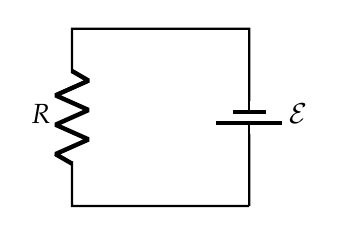
\begin{tikzpicture}[scale=1.5]
      \draw[thick](1.5,0) to[battery1,l_=$\mathcal{E}$] (1.5,1.5)--(0,1.5)
      to[R,l_=$R$] (0,0)--(1.5,0);
    \end{tikzpicture}
    \column{.75\textwidth}
    \begin{itemize}
    \item An equivalent circuit is shown on the left
    \item The amount of current can be found using Ohm's law
    \item Note that the ``motional emf'' produced is spread over the entire
      circuit
    \end{itemize}
  \end{columns}
\end{frame}

\section{Lenz's Law}

\begin{frame}
  \frametitle{Lenz's Law}
  Something very interesting happens when the current starts running on the
  wire.

  \vspace{-.2in}
  \begin{center}
    \pic{.35}{motional-emf-2.jpg}
  \end{center}
  
  \vspace{-.1in}It produces an ``induced magnetic field'' out of the page, in
  the opposite direction as the field that generated the current in the first
  place!
\end{frame}


\begin{frame}
  \frametitle{Lenz's Law}
  \begin{center}
    \fbox{
      \begin{minipage}{.7\textwidth}
        \textbf{LENZ'S LAW}\\
        The induced \emph{emf} and induced current are in such are
        direction as to oppose the change that produces them
      \end{minipage}
    }
  \end{center}

  \vspace{.2in}So basically, the conservation of energy
\end{frame}


\section{Inductance}


\begin{frame}
  \frametitle{Back \emph{emf}}
  Consider a very simple circuit consisting of a voltage source and a coil
  \begin{center}
    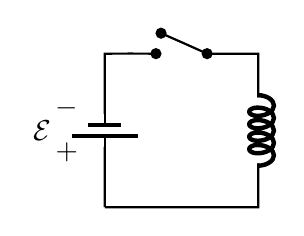
\begin{tikzpicture}[american voltages,scale=1.3]
      \draw[thick](0,0) to[battery1=$\mathcal{E}$] (0,1.5)
      to[short,-*](.5,1.5);
      \draw[thick](.55,1.7) to[short,*-*](1,1.5)--(1.5,1.5)
      to[L] (1.5,0)--(0,0);
    \end{tikzpicture}
  \end{center}
  \begin{itemize}
  \item When the switch is closed an the current begin to flow, the coil
    begin to generate a magnetic flux inside
  \item As the current changes (initially increasing with time), it
    self-induces a ``back emf'' that opposes the change in current
  \item A current can't jump from zero to some value (or from some value to
    zero) instantaneously
  \end{itemize}
\end{frame}



\begin{frame}
  \frametitle{Back \emph{emf}}
  \begin{center}
    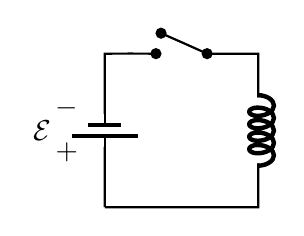
\begin{tikzpicture}[american voltages,scale=1.3]
      \draw[thick](0,0) to[battery1=$\mathcal{E}$] (0,1.5)
      to[short,-*](.5,1.5);
      \draw[thick](.55,1.7) to[short,*-*](1,1.5)--(1.5,1.5)
      to[L] (1.5,0)--(0,0);
    \end{tikzpicture}
  \end{center}
  \begin{itemize}
  \item If you try to break the circuit, you change the magnetic flux very
    rapidly
  \item Change of $\Phi$ creates a huge induced ``back emf'' that is
    proportional to $d\Phi/dt$
  \item The back emf creates a large voltage drop across the switch
  \item Large voltage across two metal contact produces a very strong electric
    field--strong enough to tear electrons away from air molecules
    (``dielectric breakdown'')
  \item Air conducts electricity in the form of a ``spark''
  \end{itemize}
\end{frame}





\begin{frame}
  \frametitle{Self Inductance}
  A solenoid carrying a current generates a magnetic field; its strength given
  by Biot-Savart law (or Amp\`{e}re's law):

  \eq{-.3in}{B=\frac{\mu_0NI}{L}}

  \vspace{-.1in}Since $\mb{B}\propto I$, the magnetic flux through the solenoid
  (really $\Phi=NBA$ where $A$ is the cross-sectional area of the solenoid and
  $N$ is the number of coils) is therefore also proportional to $I$, i.e.:

  \eq{-.3in}{\boxed{\Phi_\text{magnetic}=LI}}

  \vspace{-.1in}where $L$ is the called the \textbf{self inductance} of the
  coil.
\end{frame}


\begin{frame}
  \frametitle{Self Inductance}

  For a solenoid, we can see that the self inductance is given by:

  \eq{-.2in}{
    \boxed{L=\frac{\Phi_{\textrm{magnetic}}}{I}=\mu_0 n^2Al}
  }

  where $\mu_o$ is the magnetic permeability of free space, $n$ is the number of
  coil turns per unit length, and $A$ and $l$ are the cross-section and length
  of the solenoid. (i.e. $Al$ is the enclosed volume.)
\end{frame}


\begin{frame}
  \frametitle{Self Inductance and Induced EMF}
  If the current changes, the magnetic flux changes as well, therefore inducing
  an electromotive force in the circuit! According Faraday's law:

  \eq{-.2in}{
    \boxed{\mathcal{E}=-\frac{d\Phi}{dt}=-L\frac{dI}{dt}}
  }

  The self-induced emf is proportional to the rate of change of current.
\end{frame}


%\begin{frame}
%  \frametitle{Mutual Inductance}
%
%\end{frame}



\section{LR Circuits}

\begin{frame}
  \frametitle{Circuits with Inductors}
  \begin{itemize}
  \item Coils and solenoids in circuits are known as ``inductors'' and have
    large self inductance $L$
  \item Self inductance prevents currents rising and falling instantaneously
  \item A basic circuit containing a resistor and an inductor is called an
    \textbf{\emph{LR} circuit}:
    \begin{center}
      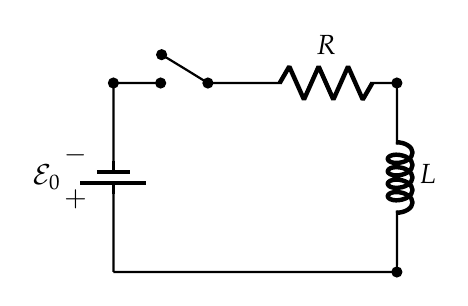
\begin{tikzpicture}[american voltages,scale=1.2]
        \draw[thick](0,0) to[battery1=$\mathcal{E}_0$,-*] (0,2)
        to[short,-*](0.5,2);
        \draw[thick](0.51,2.3) to[short,*-*](1,2)--(1.5,2) to [R=$R$,-*] (3,2)
        to [L=$L$,-*] (3,0)--(0,0);
      \end{tikzpicture}
    \end{center}
  \end{itemize}
\end{frame}

\begin{frame}
  \frametitle{Analyzing LR Circuits}
  \begin{columns}
    \column{.35\textwidth}
    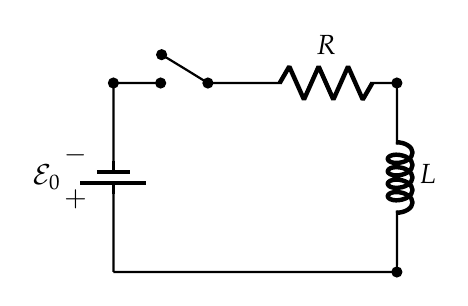
\begin{tikzpicture}[american voltages,scale=1.2]
      \draw[thick](0,0) to[battery1=$\mathcal{E}_0$,-*] (0,2)
      to[short,-*](0.5,2);
      \draw[thick](0.51,2.3) to[short,*-*](1,2)--(1.5,2) to [R=$R$,-*] (3,2)
      to [L=$L$,-*] (3,0)--(0,0);
    \end{tikzpicture}

    \column{.65\textwidth}
    Applying Kirchkoff's voltage law:

    \eq{-.2in}{\mathcal{E}_0-IR-L\frac{dI}{dt}=0}

    \vspace{-.1in}We follow the same procedure as charging a capacitor to find
    the time dependent current:

    \eq{-.2in}{I=\frac{\mathcal{E}_0}{R}\left(1-e^{-Rt/L}\right)}

    \vspace{-.15in} The time constant for an $LR$ circuit is
    
    \eq{-.2in}{\tau=\frac{L}{R}}
  \end{columns}
\end{frame}




\begin{frame}
  \frametitle{Magnetic Energy}
  Just as a capacitor stores energy, the energy stored by an inductor carrying
  a current $I$ in given by:

  \eq{-.2in}{ \boxed{U_m=\frac{1}{2}LI^2}}

  We can also define a \textbf{magnetic energy density}:

  \eq{-.2in}{ \boxed{\eta_m=\frac{B^2}{2\mu_0}}}

\end{frame}




%\section{Maxwell's Equations}
%\begin{frame}
%  \frametitle{Maxwell's Equations in Integral Form}
%  James Clerk Maxwell recognized the relationship between electricity and
%  magnetism, and combined the few laws into a unifying set of equations, now
%  known as \textbf{Maxwell's equations} for electrodynamics:
%
%
%  By manipulating the equations, we can show the existence of a
%  ``electromagnetic wave'' that travels at the speed of light.
%\end{frame}
%
%\begin{frame}
%  \frametitle{Maxwell's Equations in Differential Form}
%\end{frame}

\end{document}

